\documentclass[mathserif]{beamer}
\usepackage[sc]{mathpazo}
\usepackage[T1]{fontenc}
\usepackage[utf8]{inputenc}
\usepackage{lmodern}
\usepackage{amsfonts}
\usepackage{graphicx}
\usepackage{color}
%\usepackage{mathtools}
\newtheorem{ineq}{Inequality}
\newtheorem{eq}{Equality}
\newtheorem{target}{Target}
\newtheorem{obs}{Observation}
\usetheme{Berlin}
\useoutertheme{infolines}
\setbeamertemplate{navigation symbols}{}
%\setbeamertemplate{theorems}[numbered]
\title[Stochastic Process]{Lecture notes of Stochastic Process}
\subtitle{lectured by prof. Hsueh-I Lu}
\author{pishen}
\institute[AlgoLab]{AlgoLab, CSIE, NTU}

\begin{document}
\begin{frame}[plain]
	\titlepage
\end{frame}

\begin{frame}{Thank list}
\begin{center}
LeoSW, windker
\end{center}
\end{frame}

\begin{frame}{Stochastic Process}
	\begin{definition}
	A Stochastic process is a set of random variables $\{X(t) | t \in T\}$ where T is a index ( time) set. \\
	State Space: possible value of X(t) for each t, which is defined as subset of R.
	\end{definition}
\end{frame}

\begin{frame}{Markov Chain}
	\begin{definition}
	A Stochastic Process $\mathbb{X}$ with state space S is a Markov Chain if $\exists 0 \leq p_{ij} \leq 1 \quad \forall i,j \in S$ such that
	\begin{align*}
		(a) \quad & \sum_{j \in S} p_{ij} = 1 \quad \forall i \in S \\
		(b) \quad & P(X(t+1) = j | X(0) = i_0, X(1) = i_1, ..., X(t) = i) = p_{ij} \\
			& \quad \forall t, i_0,i _1, ..., i_{t-1}
	\end{align*}
	$\mathbb{P}$ denotes the matrix form of $p_{ij}$ with sum of any row is 1.
	\end{definition}
	Lemma: $P(X(n) = j | X(0) = i) = \mathbb{P}^n[i, j]$
\end{frame}

\begin{frame}{Proof of lemma}
	We know statement is true for $(m+n) = 0$. For $(m+n) > 0$: 
	\begin{align*}
	P(X&(m+n) = j | X(0) = i) \\
		\text{{\color{brown}=} }& \sum_{k \in S} P(X(m+n) = j \text{ and } X(m) = k | X(0) = i) \\
		\text{{\color{blue}=} }& \sum_{k \in S} P(X(m+n) = j | X(m) = k \text{ and } X(0) = i) \cdot \\
			& P(X(m) = k | X(0) = i) \\
		\text{{\color{green}=} }& \sum_{k \in S} P(X(m+n) = j | X(m) = k) \cdot P(X(m) = k | X(0) = i) \\
		\text{{\color{red}=} }& \sum_{k \in S} P^n[k, j] \cdot P^m[i, k] \\
		=& \sum_{k \in S} P^m[i, k] \cdot P^n[k, j] \\
		=& \mathbb{P}^n[i, j]
	\end{align*}
\end{frame}

\begin{frame}{Proof of lemma(cont)}

	{\color{brown}= }: conditional on $X(m)$ \\
	{\color{blue}= }: definition of conditional probability \\
	{\color{green}= }: (see next page) \\
	{\color{red}= }: inductive hypothesis
\end{frame}

\begin{frame}{Proof of lemma(cont)}
	\begin{align*}
	P(X&(m+n) = j | X(m) = k \text{ and } X(0) = i) \\
		\text{{\color{blue}=} }& \sum_{r \in S} P(X(m+n) = j | \\
			& X(m+n-1) = r \text{ and } X(m) = k \text{ and } X(0) = i) \cdot \\
 			& P(X(m+n-1) = r | X(m) = k \text{ and } X(0) = i)\\
		\text{{\color{brown}=} }& \sum_{r \in S} P(X(m+n) = j | X(m+n-1) = r) \cdot \\
			& P(X(m+n-1) = r | X(m) = k) \\
		=& P(X(m+n) = j | X(m) = k)
	\end{align*}
	{\color{blue}=}: conditional on $X(m+n-1)$ \\
	{\color{brown}=}: first part by definition of Markov chain and second part by inductive hypothesis \\
\end{frame}

\begin{frame}{Absorbing State}
	Let $\mathbb{A}$ be a set of accepting states. We would like to know the probability that $\mathbb{X}$ has ever entered some state in $\mathbb{A}$. Technique: merge all state of $\mathbb{A}$ into a new absorbing state a. Set matrix of $\mathbb{X}$ by once enter a, then probability of a goes to a is 1.
\end{frame}

\begin{frame}{Recurrent \& transient}
	\begin{definition}
	The \textit{recurrent probability} of state $i$ of Markov chain $\mathbb{X}$ is 
	\[
	f_i = P(\text{there exists an index}~t \geq 1~\text{with}~X(t)=i | X(0)=i)
	\]
	\begin{itemize}
	\item State $i$ of $\mathbb{X}$ is \textit{recurrent} if $f_i = 1$.
	\item State $i$ of $\mathbb{X}$ is \textit{transient} if $f_i < 1$.
	\end{itemize}
	\end{definition}
\end{frame}

\begin{frame}{Recurrent \& transient (cont.)}
	\begin{itemize}
	\item If state $i$ is recurrent, by the property of Markov chain, 
		once it re-enter the state $i$, we can take it as starting from $X(0)$ again. \\
		Hence we know that it will keep re-entering the state $i$ again and again in the process.
	\item If state $i$ is transient, in each period it start going from $i$,
		it may have probability $1 - f_i$ that it won't come back anymore. \\
		Hence the probability that the process will be in state i for exactly $n$ periods equals
		${f_i}^{n-1}(1-f_i), ~n \geq 1$, which is a geometric distribution.
	\end{itemize}
\end{frame}

\begin{frame}{Recurrent \& transient (cont.)}
	\begin{itemize}
	\item From the preceding page, it follows that state $i$ is recurrent if and only if,
		starting in state $i$, the expected number of steps that the process is in state $i$ is infinite.
	\item We can also derive that, if the Markov chain has finite states, at least one state is recurrent.
	\end{itemize}
\end{frame}

\begin{frame}{Expected number of visits}
	Let 
	\[
	I(n) = \left\{
	\begin{array}{l l}
		1 & ~\text{if $X(n) = i$}\\
		0 & ~\text{if $X(n) \neq i$} \\
	\end{array} \right.
	\]
	we have $\sum_{n=0}^\infty I(n)$ represents the number of steps that the process is in state $i$, and
	\begin{align*}
	E\left[ \sum_{n=0}^\infty I(n)|X(0) = i \right] & = \sum_{n=0}^\infty E[I(n)|X(0)=i] \\
	& = \sum_{n=0}^\infty 1 \cdot P(X(n)=i|X(0)=i) \\
	& = \sum_{n=0}^\infty P^n_{ii}
	\end{align*}
	We set $T = \sum_{n=0}^\infty I(n)$
\end{frame}

\begin{frame}{Lemma 1}
	From the above statements, we prove the following
	\begin{lemma}
	State $i$ is 
	\[
	\text{recurrent } \iff \sum_{n=0}^\infty P^n_{ii} = \infty \text{,}
	\]
	\[
	\text{transient } \iff \sum_{n=0}^\infty P^n_{ii} < \infty
	\]
	\end{lemma}
\end{frame}

\begin{frame}{Proof of Lemma 1}
	($\Rightarrow$:)\\
	($\Leftarrow$:)\\
	Suppose state i is transient($f_i < 1$), consider $P(T=k) = f_i^{k-1} \cdot (1-f_i)$. Since T is a geometric distribution, we have
	\begin{align*}
		E[T] 	&= \sum_{k = 0}^\infty k \cdot f_i^{k-1} \cdot f_i \\
			&=\frac{1}{1-f_i} < \infty
	\end{align*}
\end{frame}

\begin{frame}{Communicated states}
	\begin{definition}
	State $i$ and $j$ \textit{communicate}, denoted $i \leftrightarrow j$,
	if there exist integers $m \geq 0$ and $n \geq 0$ such that
	\[
	P^m_{ij} > 0 \text{ and } P^n_{ji} > 0
	\]
	We say a Markov chain $\mathbb{X}$ is irreducible if $i \leftrightarrow j \quad \forall i, j \in S$
	\end{definition}
\end{frame}

\begin{frame}{Lemma 2}
	\begin{lemma}
	If $i \leftrightarrow j$, then the following statements hold.
	\begin{itemize}
	\item State $i$ is recurrent if and only if state $j$ is recurrent.
	\item State $i$ is transient if and only if state $j$ is transient.
	\end{itemize}
	Corollary: $\mathbb{X}$ is finite and irreducible $\implies$ all states are recurrent.
	\begin{itemize}
	\item $\mathbb{X}$ is finite $\implies \exists i \in S$ is recurrent (proof later)
	\item By Lemma 2, all states are recurrent
	\end{itemize}
	\end{lemma}
\end{frame}

\begin{frame}{Proof}
	Let $m$ and $n$ be nonnegative integers with $P^m_{ij},  P^n_{ji} > 0$.
	Suppose that state $j$ is recurrent, i.e., $\sum_{t=0}^\infty P^t_{jj} = \infty$.
	We have
	\begin{align*}
	\sum_{t=0}^\infty P^t_{ii} & \geq \sum_{t=0}^\infty P^{m+t+n}_{ii} \\
	& \geq \sum_{t=0}^\infty P^m_{ij} \cdot P^t_{jj} \cdot P^n_{ji} \\
	& = P^m_{ij} \cdot P^n_{ji} \cdot \sum_{t=0}^\infty P^t_{jj} = \infty
	\end{align*}
	Thus, state $i$ is also recurrent.
\end{frame}

\begin{frame}{Infinite drunken man problem}
	\begin{center}
	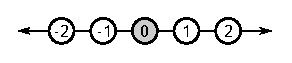
\includegraphics[width=0.6\textwidth]{infinite_drunken.eps}
	\end{center}
	Let the state space consist of all integers.
	Let $X(0) = 0$ (i.e. at time 0 the drunken man is in state 0).
	The transition probabilities are such that
	\[
	P_{i, (i+1)} = P_{i, (i-1)} = 0.5
	\]
	holds for all states $i$ of $\mathbb{X}$.
\end{frame}

\begin{frame}{Gambler's ruin}
\end{frame}

\begin{frame}{Outline}
	\begin{enumerate}
		\item Limiting probabilities
		\item Stationary distribution
		\item Long-run proportion
		\item (Inverse of) Expected return time
	\end{enumerate}
\end{frame}

\begin{frame}{Limiting Probabilities}
	\begin{definition}
		Number $\pi_j$ is the \textit{limiting probability} of $j$ if
		\[
		\pi_j = \lim_{n \to \infty} P^n_{ij}
		\]
		holds for all states $i \in S$ ($S \subseteq \mathbb{N}$ is the state space).
	\end{definition}
	\begin{itemize}
		\item $\pi_j$ is independent of $i$.
		\item $\lim_{n \to \infty} P^n = 
			\begin{pmatrix}
				\pi \\
				\pi \\
				\vdots
			\end{pmatrix}$
			, where $\pi = (\pi_1, \pi_2, \ldots)$
	\end{itemize}
\end{frame}

\begin{frame}{Stationary Probability Distribution}
	\begin{definition}
		Non-negative row vector $\pi = (\pi_1, \pi_2, \ldots)$
		is a \textit{stationary probability distribution} of $\mathbb{X}$
		if $\pi \times P = \pi$ holds and $\sum_{i \in S} \pi_i = 1$
	\end{definition}
	\begin{itemize}
		\item $\pi$ is a normalized left eigenvector with eigenvalue $=1$.
		\item If $X(0)$ has distribution $\pi$, then $X(t)$ has the same distribution $\pi$
			for all $t \geq 1$.
			$\pi$ is also called as \textit{steady-state distribution}.
		\item It doesn't mean that each $X(t)$ become independent.
			$\pi$ only means the distribution of $X(t)$ when the previous random variable's value is unknown.
	\end{itemize}
\end{frame}

\begin{frame}{Theorem 1}
	\begin{theorem}
		Let $\mathbb{X}$ be an \textit{irreducible}, \textit{aperiodic}, \textit{positive recurrent} Markov chain, then
		\begin{itemize}
			\item The limiting probability $\pi_j$ of each state $j$ exists.
			\item $\pi = (\pi_1, \pi_2, \ldots)$ is the unique stationary probability distribution.
		\end{itemize}
	\end{theorem}
	\begin{itemize}
		\item The proof will be stated at page \hyperlink{thm1_proof}{\pageref{thm1_proof}}.
	\end{itemize}
\end{frame}

\begin{frame}{Expected return time}
	\begin{definition}
		The \textit{expected return time} of state $i \in S$ is
		\[
		\mu_i = \sum_{n \geq 1} n \cdot f_i^{(n)}
		\]
		where
		\[
		f_i^{(n)} = P(\min\{t:X(t) = i, t\geq 1\} = n | X(0) = i)
		\]
	\end{definition}
	\begin{itemize}
		\item $f_i = \sum_{n \geq 1} f_i^{(n)}$
	\end{itemize}
\end{frame}

\begin{frame}{Positive recurrent \& null recurrent}
	\begin{definition}
		State $i$ is \textit{positive recurrent} if $\mu_i < \infty$
	\end{definition}
	\begin{definition}
		State $i$ is \textit{null recurrent} if $\mu_i = \infty$
	\end{definition}
	\begin{itemize}
		\item Both are recurrent states, and are \textit{class properties}, which means that if state $i$ and $j$ communicate, they will share this property.
		\item If $\mathbb{X}$ is finite, then each recurrent state of $\mathbb{X}$ is positive recurrent.\\
			Proof stated at page \pageref{finite_pos_rec}.
	\end{itemize}
\end{frame}

\begin{frame}{Example of null recurrent}
	\begin{example}
		For a Markov chain with $n$ states ($1,\ldots,n$), if 
		\[
		P(X(t+1)=i+1|X(t)=i) = 1-1/n
		\]
		and
		\[
		P(X(t+1)=1|X(t)=i) = 1/n
		\]
		According to geometric distribution (taking $p = 1/n$), the expectation value of ``steps taken for state 1 to come back'' will be $1/p = n$, hence $\lim_{n\to\infty} n = \infty$.
	\end{example}
\end{frame}

\begin{frame}{Period of a chain}
	\begin{definition}
		The \textit{period} of state $i$ is $d$ if $d$ is the largest integer such that
		\[
		P^n_{ii} = 0
		\]
		holds for all $n$ which is not divisible by $d$.
	\end{definition}
	\begin{definition}
		If each state of $\mathbb{X}$ has period 1, then $\mathbb{X}$ is called \textit{aperiodic}.
	\end{definition}
	\begin{itemize}
		\item If $P_{ii} > 0$ for all $i \in S$, then $\mathbb{X}$ is aperiodic.
		\item Period can be seen as the $\gcd$ of all $n$ that have $P^n_{ii} > 0$, note that $P^{\gcd}_{ii} > 0$ is not necessary.
		\item The period of drunken man problem is 2.
	\end{itemize}
\end{frame}

\begin{frame}{Lemma 1}
	\begin{lemma}
		If state $j$ has period $1$ and is positive recurrent, then
		\[
		\pi_{ij} \equiv \lim_{n \to \infty} P^n_{ij}
		\]
		exists and is positive for all states $i \in S$.
	\end{lemma}
	\begin{itemize}
		\item This can be proved by the Blackwell theorem in Renewal theory.
		\item It doesn't promise that $\pi_{ij} = \pi_{i'j}$ for any $i,i' \in S$.
			But they will be the same if we add the irreducible property ($i \leftrightarrow i'$).
	\end{itemize}
\end{frame}

\begin{frame}{Property of $\lim$}
	\begin{itemize}
		\item The position of $\lim$ may not be switched arbitrarily in an equation.
			\begin{example}
				\[
				1 = \lim_{n \to \infty}\lim_{m \to \infty} \frac{m}{m+n} \neq
				\lim_{m \to \infty}\lim_{n \to \infty} \frac{m}{m+n} = 0
				\]
			\end{example}
		\item $\lim$ would not influence the inequality.
			\begin{example}
				\begin{center}
					If $f(n) \geq g(n)$, then
					$\lim_{n \to \infty} f(n) \geq \lim_{n \to \infty} g(n)$
				\end{center}
			\end{example}
	\end{itemize}
\end{frame}

\begin{frame}{Property of $\lim$ (cont.)}
	\begin{itemize}
		\item $\lim$ is linear operator under finite number of functions.
	\end{itemize}
	\begin{example}
		For $m < \infty$,
		\[
		\sum_{i=1}^m \lim_{n \to \infty} f_i(n) = \lim_{n \to \infty} \sum_{i=1}^m f_i(n)
		\]
	\end{example}
	\textcolor{red}{need an example of $m = \infty$}
%	\begin{itemize}
%		\item It may not work if we push $m$ to $\infty$ first, since $\sum_{i=1}^m f_i(n)$ may influence the result.
%			For example, if $1 \leq i \leq n, f_i(n) = 1/n$, then LHS will be 0, while RHS will be 1.
%			But pushing $m$ to $\infty$ after pushing $n$ to $\infty$ first is OK.
%	\end{itemize}
\end{frame}

\begin{frame}{Inequality 1}
	\begin{ineq}
		\[
		\sum_{j \in S} \pi_{ij} \leq 1 \quad\forall i \in S
		\]
	\end{ineq}
\end{frame}

\begin{frame}{Proof}
		\begin{align*}
			\lim_{m \to \infty} \sum_{j=1}^m \pi_{ij} &= \lim_{m \to \infty} \sum_{j=1}^m \lim_{n \to \infty} P^n_{ij} \\
			&= \lim_{m \to \infty} \lim_{n \to \infty} \sum_{j=1}^m P^n_{ij} \\
			&\leq \lim_{m \to \infty} \lim_{n \to \infty} \sum_{j \in S} P^n_{ij} = 1
		\end{align*}
	\begin{itemize}
		\item The last equation works since $\sum_{j \in S} P^n_{ij} = 1$.
	\end{itemize}
\end{frame}

\begin{frame}{Inequality 2}
	\begin{ineq}
		For state $j \in S$, we have
		\[
		\pi_{ij} \geq \sum_{k \in S} \pi_{ik} P_{kj}
		\]
	\end{ineq}
\end{frame}

\begin{frame}{Proof}
	For $m \geq 1$ and $n \geq 1$,
	\[
	P^{n+1}_{ij} = \sum_{k \in S} P^n_{ik} P_{kj} \geq \sum_{k=1}^m P^n_{ik} P_{kj}
	\]
	then
	\[
	\pi_{ij} = \lim_{n \to \infty} P^{n+1}_{ij}
		\geq \lim_{n \to \infty} \sum_{k=1}^m P^n_{ik} P_{kj} 
		 = \sum_{k=1}^m \lim_{n \to \infty} P^n_{ik} P_{kj} 
		 = \sum_{k=1}^m \pi_{ik} P_{kj}
	\]
	hence, we know
	\[
	\lim_{m\to\infty} \pi_{ij} = \pi_{ij} \geq 
	\lim_{m\to\infty}\sum_{k=1}^m \pi_{ik}P_{kj} = \sum_{k\in S} \pi_{ik}P_{kj}
	\]
\end{frame}

\begin{frame}{Equality 1}
	\begin{eq}
		\[
		\pi_{ij} = \sum_{k \in S} \pi_{ik} P_{kj}
		\]
	\end{eq}
\end{frame}

\begin{frame}{Proof}

		Assume for contradiction $\pi_{ij} > \sum_{k \in S} \pi_{ik} P_{kj}$, then
		\begin{align*}
		\lim_{m\to\infty}\sum_{j=1}^m & > \lim_{m\to\infty}\sum_{j=1}^m 
		\lim_{p\to\infty}\sum_{k=1}^p \pi_{ik}P_{kj} \\
		& = \lim_{m\to\infty}\lim_{p\to\infty}\sum_{j=1}^m \sum_{k=1}^p \pi_{ik}P_{kj} \\
		& = \lim_{m\to\infty}\lim_{p\to\infty}\sum_{k=1}^p \pi_{ik} \sum_{j=1}^m P_{kj} \\
		& = \lim_{p\to\infty}\sum_{k=1}^p \pi_{ik} \lim_{m\to\infty}\sum_{j=1}^m P_{kj} \\
		& = \lim_{p\to\infty}\sum_{k=1}^p \pi_{ik} \cdot 1 = \lim_{p\to\infty}\sum_{k=1}^p \pi_{ik}
		\end{align*}
		
%		\begin{align*}
%			\sum_{j \in S} \pi_j &> \sum_{j \in S}\sum_{i \in S} \pi_i P_{ij} \\
%			&= \sum_{i \in S} \pi_i \sum_{j \in S} P_{ij} = \sum_{i \in S} \pi_i
%		\end{align*}
		

%	\begin{itemize}
%		\item $\sum$ should be represented by $\lim \sum$, the equation will still work.
%		\item \textcolor{red}{why the proof work when switching $\sum_{j \in S} \& \sum_{i \in S}$?}
%	\end{itemize}
\end{frame}

\begin{frame}{Proof (cont.)}
\begin{itemize}
\item Since a value cannot be greater than itself, we got contradiction.
\item In the 4th line, two $\lim$ can be switched because the value can only get larger when applying $\lim$ on it. \textcolor{red}{not sure}
\end{itemize}
\end{frame}

\begin{frame}{Proof of theorem 1}\label{thm1_proof}
	\begin{itemize}
		\item \textbf{Step 0}: existence of limiting probability.
		\item \textbf{Step 1}: existence of stationary probability distribution.
		\item \textbf{Step 2}: uniqueness.
	\end{itemize}
\end{frame}

\begin{frame}{0. Existence of limiting probability}
	\begin{proof}
		By lemma 1, we know that there exists a $\pi_j$ for row $i$.
		Since the Markov chain is irreducible and all the states are positive recurrent, 
		for any state $i'$ other than $i$, we know that $i'$ surely will visit $i$ in finite steps.
		Therefore, the $\pi_j$ value at row $i'$ will equal to the $\pi_j$ value at row $i$,
		which means that all the $\pi_j$ for column $j$ are the same, and is the limiting probability.
	\end{proof}
	\textcolor{red}{still not clear enough}
\end{frame}

\begin{frame}{1. Existence of stationary probability distribution}\label{existence}
	We want to prove that
	\begin{target}
		There's a vector $s = (s_1, s_2, \ldots)$ such that
		\begin{enumerate}
			\item $\sum_{i \in S} s_i = 1$
			\item $s \times P = s$
		\end{enumerate}
	\end{target}
\end{frame}

\begin{frame}
	\begin{proof}
		By lemma 1, we know that there exists a $\pi = (\pi_1, \pi_2, \ldots)$. \\
		And by equality 1, we know that
		\[
		(\pi_1, \pi_2, \ldots) \times P = (\pi_1, \pi_2, \ldots)
		\]
		Hence $\pi$ can satisfy the 2nd part of our target. \\
		Then, we take $k = \sum_{i \in S} \pi_i$.
		By inequality 1, we know that $k < \infty$, and can get
		\[
		(\frac{\pi_1}{k}, \frac{\pi_2}{k}, \ldots) \times P = (\frac{\pi_1}{k}, \frac{\pi_2}{k}, \ldots)
		\]
		where $\sum_{i \in S} \frac{\pi_i}{k} = 1$ also satisfy the 1st part of our target. \\
		Therefore, this vector can be $s$, which means that it exists.
	\end{proof}
\end{frame}

\begin{frame}{2. Uniqueness}\label{uniqueness}
	\begin{target}
		If $s = (s_1, s_2, \ldots)$ is a stationary distribution of $\mathbb{X}$, then $s = \pi$.
	\end{target}
	\begin{itemize}
		\item We'll prove this by inequality 3 \& 4.
	\end{itemize}
\end{frame}

\begin{frame}{Inequality 3}
	\begin{ineq}
		\[
		s_j \geq \pi_j, \forall j \in S
		\]
	\end{ineq}
\end{frame}

\begin{frame}
	\begin{proof}
		Let the distribution of $X(0)$ be $s$, by the property of stationary distribution, we have
		\begin{align*}
			             s_j &= P(X(n)=j) = \sum_{i \in S} P(X(n) = j | X(0) = i)P(X(0) = i) \\
			                 &= \sum_{i \in S} P^n_{ij} \cdot s_i \\
			                 &\geq \sum_{i=1}^m P^n_{ij} \cdot s_i \\
			\Rightarrow  s_j &= \lim_{m \to \infty}\lim_{n \to \infty} s_j \\
			                 &\geq \lim_{m \to \infty}\lim_{n \to \infty} \sum_{i=1}^m P^n_{ij} \cdot s_i
			                  = \lim_{m \to \infty}\sum_{i=1}^m \pi_j \cdot s_i = \pi_j
		\end{align*}
	\end{proof}
\end{frame}

\begin{frame}{Inequality 4}
	\begin{ineq}
		\[
		s_j \leq \pi_j, \forall j \in S
		\]
	\end{ineq}
\end{frame}

\begin{frame}
	\begin{proof}
		Similar in the proof above, $\forall m,n \geq 1$, we have
		\begin{align*}
			            s_j &= \sum_{i \in S} P^n_{ij} \cdot s_i \\
			                &\leq \sum_{i=1}^m P^n_{ij} \cdot s_i + \sum_{i=m+1}^\infty s_i \\
			\Rightarrow s_j &= \lim_{m \to \infty}\lim_{n \to \infty} s_j \\
			                &\leq \lim_{m \to \infty}\lim_{n \to \infty} \left( 
			                	\sum_{i=1}^m P^n_{ij} \cdot s_i + \sum_{i=m+1}^\infty s_i \right) \\
			                &= \pi_j
		\end{align*}
	\end{proof}
\end{frame}

\begin{frame}{An example Markov chain}
	\begin{example}
		\[
		P = 
		\begin{pmatrix}
			\alpha & 1 - \alpha \\
			\beta  & 1 - \beta
		\end{pmatrix},
		0 < \alpha, \beta < 1
		\]
		\[
		\pi = \left( \frac{\beta}{1+\beta-\alpha}, \frac{1-\alpha}{1+\beta-\alpha} \right) 
		\]
	\end{example}
\end{frame}

\begin{frame}{Real world example: Hardy-Weinberg Law}
	\begin{example}
		There're two kinds of allele: 
		\begin{itemize}
			\item dominant: \textbf{A}
			\item recessive: \textbf{a}
		\end{itemize}
		And three kinds of senotype with population proportion as follow:
		\begin{itemize}
			\item AA: $p$
			\item aa: $q$
			\item Aa: $r = 1 - (p + q)$
		\end{itemize}
	\end{example}
\end{frame}

\begin{frame}
	\begin{example}[cont.]
		\[
		P = 
		\bordermatrix{ ~ & AA                      & aa                      & Aa            \cr
			            AA & p+\frac{r}{2}           & 0                       & q+\frac{r}{2} \cr
			            aa & 0                       & q+\frac{r}{2}           & p+\frac{r}{2} \cr
			            Aa & \frac{p}{2}+\frac{r}{4} & \frac{p}{2}+\frac{r}{4} & \frac{p+q+r}{2} \cr}
		\]
		we get $\pi = (p, q, r)$ when
		\begin{itemize}
			\item $p = {\left( p + \frac{r}{2} \right)}^2$
			\item $q = {\left( q + \frac{r}{2} \right)}^2$
			\item $r = 2 \left( p + \frac{r}{2} \right)\left( q + \frac{r}{2} \right)$
		\end{itemize}
	\end{example}
\end{frame}

\begin{frame}{Long-run proportion}
	\begin{definition}
		We say that $r_j$ is the \textit{long-run proportion} of state $j \in S$ if
		\[
		r_j = \lim_{n\to\infty} \frac{1}{n} \sum_{1 \leq t \leq n} P^t_{ij}
		\]
		holds for each state $i \in S$.
	\end{definition}
	\begin{itemize}
		\item It represents the average appearance times of state $j$ in the whole process.
		\item We will show that (in theorem 3) if $\mathbb{X}$ is irreducible, then the long-run proportion of all states exist.
	\end{itemize}
\end{frame}

\begin{frame}{Theorem 2}
	\begin{theorem}[type 1]
	If $r_j$ exists for each $j \in S$ and $\sum_{j \in S} r_j > 0$,
	then $r = (r_1, r_2, \ldots)$ is the unique stationary distribution of $\mathbb{X}$.
	\end{theorem}
	or
	\begin{theorem}[type 2]
	If $r_j$ exists for each $j \in S$ and \textbf{a stationary distribution exists},
	then $r = (r_1, r_2, \ldots)$ is the unique stationary distribution of $\mathbb{X}$.
	\end{theorem}
\end{frame}

\begin{frame}[shrink]{Proof}
	\textbf{Existence of stationary distribution in type 1:} \\
	Let 
	\[
	R = 
	\begin{pmatrix}
		r \\
		r \\
		\vdots
	\end{pmatrix} 
	= \lim_{n\to\infty} \frac{1}{n} \sum_{1 \leq t \leq n} P^t
	\]
	then
	\begin{align*}
		R \times P &= \lim_{n\to\infty} \frac{1}{n} \sum_{1 \leq t \leq n} P^{t+1} \\
		&= \lim_{n\to\infty} \frac{1}{n} \sum_{1 \leq t \leq n} P^t + \lim_{n\to\infty} \frac{1}{n}(P^{n+1} - P) \\
		&= R
	\end{align*}
	As stated later, $\sum_{j \in S} r_j \leq 1$, hence by normalizing $r$, we prove that stationary distribution exist.
	\begin{itemize}
	\item \textcolor{red}{$(\lim f(n))\cdot g(n) = \lim f(n) \cdot g(n)$?}
	\item \textcolor{red}{can replace the proof on page \pageref{existence}?}
	\end{itemize}
\end{frame}

\begin{frame}{Proof (cont.)}
	\textbf{Uniqueness:} \\
	Let $\pi$ be an arbitrary stationary distribution, then
	\begin{align*}
	r &= \pi \times R \\
	&= \pi \times \lim_{n\to\infty} \frac{1}{n} \sum_{1 \leq t \leq n} P^t \\
	&= \lim_{n\to\infty} \frac{1}{n} \sum_{1 \leq t \leq n} \pi \times P^t \\
	&= \lim_{n\to\infty} \frac{1}{n} \sum_{1 \leq t \leq n} \pi \\
	&= \pi
	\end{align*}
	\textcolor{red}{can replace the proof for page \pageref{uniqueness}?}
\end{frame}

\begin{frame}{Proof (cont.)}\label{proportion_sum}
	\textbf{Prove that $\sum_{j \in S} r_j \leq 1$:}\\
	\begin{align*}
	\sum_{j \in S} r_j & = 
	\lim_{m\to\infty} \sum_{j=1}^m \lim_{n\to\infty} \frac{1}{n} \sum_{t=1}^n P^t_{ij} \\
	& = \lim_{m\to\infty} \lim_{n\to\infty} \frac{1}{n}\sum_{t=1}^n \sum_{j=1}^m P^t_{ij} \\
	& \leq \lim_{m\to\infty} \lim_{n\to\infty} \frac{1}{n}\sum_{t=1}^n \sum_{j\in S} P^t_{ij} \\
	& = \lim_{m\to\infty} \lim_{n\to\infty} \frac{1}{n}\sum_{t=1}^n 1 = 1
	\end{align*}
\end{frame}

\begin{frame}{Example 1}
	On a highway, if we know the probability that
	\begin{itemize}
	\item A truck is followed by a truck: $1/4$
	\item A truck is followed by a car: $3/4$
	\item A car is followed by a truck: $1/5$
	\item A car is followed by a car: $4/5$
	\end{itemize}
	We can construct a matrix
	\[
	\bordermatrix{~ & T   & C   \cr
                  T & 1/4 & 3/4 \cr
                  C & 1/5 & 4/5 \cr}
	\]
	and get the portion of trucks and cars on the whole highway as the eigenvector $(4/19, 15/19)$
	(we will know that long-run proportion exists by Theorem 3).
\end{frame}

\begin{frame}{Example 2}
	For a system which has several good and bad states, we have a matrix $P$:
	\[
	\bordermatrix{~      & g_1 & g_2 & \cdots & b_1 & b_2 & \cdots \cr
                  g_1    &     &     &        &     &     &        \cr
                  g_2    &     &     &        &     &     &        \cr
                  \vdots &     &     &        &     &     &        \cr
                  b_1    &     &     &        &     &     &        \cr
                  b_2    &     &     &        &     &     &        \cr
                  \vdots &     &     &        &     &     &        \cr}
	\]
\end{frame}

\begin{frame}{Example 2 (cont.)}
	\textbf{Q1:} Breakdown rate (breakdown times $/$ total time)\\
	The long-run frequency of going to a bad state from a good state is
	\[
	\sum_{i \in g} \sum_{j \in b} r_i P_{ij}
	\]
\end{frame}

\begin{frame}{Example 2 (cont.)}
	\textbf{Q2:} The expected time $\mu_G$ (resp. $\mu_B$) of staying in good (resp. bad) states once we reach a good (resp. bad) state? \\
	\textbf{Ans:} \\
	For each $t = 1, 2, \ldots$, let $G_t$ (resp. $B_t$) be the length of the $t$-th good (resp. bad) phase of consecutive good (resp. bad) states.
	By the strong law of large numbers, 
	\[
	P\left( \lim_{t\to\infty} \frac{G_1 + B_1 + G_2 + B_2 + \cdots + G_t + B_t}{t} = \mu_G + \mu_B \right) = 1
	\]
	Since the reciprocal of above is the breakdown rate, we get equation (1):
	\[
	P\left( \sum_{i \in G} \sum_{j \in B} \pi_i P_{ij} = \frac{1}{\mu_G + \mu_B} \right) = 1
	\]
\end{frame}

\begin{frame}{Example 2 (cont.)}
	Also, with probability 1, we get equation (2):
	\[
	P\left( \sum_{i \in G} r_i = 
	\lim_{t\to\infty}\frac{G_1 + G_2 + \cdots + G_t}{G_1 + B_1 + \cdots + G_t + B_t}
	= \frac{\mu_G}{\mu_G + \mu_B} \right) = 1
	\]
	Then, by $(2)/(1)$, we get that
	\[
	P\left( \mu_G = \frac{\sum_{i \in G} r_i}{\sum_{i \in G}\sum_{j \in B} r_i P_{ij}} \right) = 1
	\]
	\begin{itemize}
	\item \textcolor{red}{$\lim \frac{f(n)}{g(n)} = \frac{\lim f(n)}{\lim g(n)}$?}
	\end{itemize}
\end{frame}

\begin{frame}{Theorem 3}\label{pro_value}
	\begin{theorem}
	If $\mathbb{X}$ is irreducible, then the long-run proportion $r_i$ exists with probability $1$, moreover,
	\begin{enumerate}
	\item If state $i$ is positive recurrent (i.e. $0 < \mu_i < \infty$), then $P(r_i = \frac{1}{\mu_i}) = 1$.
	\item If state $i$ is null recurrent (i.e. $\mu_i = \infty$) or transient, then $P(r_i = 0) = 1$.
	\end{enumerate}
	where $\mu_i$ is the expected return time of state $i$
	\end{theorem}
\end{frame}

\begin{frame}{Proof}
	\textbf{Part 1:} \\
	Suppose $X(0) = i$, $T_k$ is the number of steps required for the $k$-th $i$ goes to $(k+1)$-st $i$,
	then by the strong law of large number,
	\begin{align*}
	&P\left( \lim_{k\to\infty} \frac{T_1 + T_2 + \cdots + T_k}{k} = \mu_i \right) = 1 \\
	\Rightarrow & P\left( r_i = \lim_{k\to\infty} \frac{k}{T_1 + T_2 + \cdots + T_k} = \frac{1}{\mu_i} \right) = 1
	\end{align*}
	\begin{itemize}
	\item \textcolor{red}{$\lim (A/B) = \frac{1}{\lim (B/A)}$?}
	\end{itemize}
\end{frame}

\begin{frame}{Proof (cont.)}
	\textbf{Part 2:} \\
	\begin{enumerate}
	\item If $i$ is transient, $i$ will only appear finite times in the long-run, hence
		\[
		r_i = \frac{finite}{\infty} = 0
		\]
	\item If $i$ is null recurrent, $\mu_i$ is $\infty$, then
		\[
		P\left( \lim_{k\to\infty} \frac{T_1 + T_2 + \cdots + T_k}{k} = \infty \right) = 1
		\]
		\[
		P\left( r_i = \lim_{k\to\infty} \frac{k}{T_1 + T_2 + \cdots + T_k} = 0 \right) = 1
		\]
		(The first equation is not promised by the strong law of large number.
		But if it's not $\infty$, we can say that $\mu_i$ is not $\infty$, which is a contradiction.)
	\end{enumerate}
\end{frame}

\begin{frame}{Example 1}\label{finite_pos_rec}
	\begin{example}[type 1]
	If $\mathbb{X}$ is \textbf{irreducible} and finite, then $\mathbb{X}$ has no null recurrent states.
	\end{example}
	\begin{example}[type 2]
	If $\mathbb{X}$ is finite, then $\mathbb{X}$ has no null recurrent states.
	\end{example}
	\begin{itemize}
	\item Finite irreducible imply positive recurrent.
	\end{itemize}
\end{frame}

\begin{frame}{Proof}
	\begin{itemize}
	\item \textbf{Type 1:}\\
		If there's a state which is null recurrent, by irreducible, all the states will be null recurrent.
		Then, all states have $P(r_i = 0) = 1$.
		By changing the proof in page \pageref{proportion_sum} into finite states version, 
		we know that $\sum r_i = 1$.
		So it's impossible for finite $r_i$, which are all close to 0, to sum up to 1.
	\item \textbf{Type 2:}\\
		If it's not irreducible, the finite set of communicated null recurrent states still form an irreducible and finite Markov chain, which can fit the requirement of type 1.
	\end{itemize}
\end{frame}

\begin{frame}{Example 2}
	\begin{example}
	In the drunken man problem with infinite states, no state will be positive recurrent.
	\end{example}
	\begin{itemize}
	\item Infinite drunken man imply no positive recurrent.
		Note that it doesn't mean all infinite irreducible Markov chain has no positive recurrent state.
	\end{itemize}
\end{frame}

\begin{frame}{Proof}
	If all the states are positive recurrent, then by theorem 3, 
	we know that all the $r_i > 0$ and is a finite value.
	Since each state of drunken man problem has the same structure, all the $r_i$ has same value.
	We then set $r = \epsilon\cdot r_i$ ($0 < \epsilon < 1$) such that 
	$r_i > r > 0, \forall i$.
	And get
	\[
	\sum_{i\in S} r_i > \sum_{i\in S} r = \infty > 1
	\]
	which is contradiction to \hyperlink{proportion_sum}{page \pageref{proportion_sum}}.
\end{frame}

\begin{frame}{Example 3: Poisson Hotel}
	\begin{example}
	There's a hotel, with $N$ representing the number of newly occupied rooms each day ($N$ is a poisson distribution with parameter $\lambda$).
	And the number of consecutive check-in days of each room is a geometric distribution with probability $p$ ($p$ is the probability of check-out).
	$X(t)$ is the number of occupied rooms in day $t$.
	\end{example}
\end{frame}

\begin{frame}{\textbf{Q1:} $P_{ij} = $?}
	We set $R_i$ as a binomial distribution with parameter $(i, 1-p)$, which represents the number of rooms which will remain occupied in the next day, then
	\begin{align*}
	P_{ij} & = P(R_i + N = j) \\
	& = \sum_{k\geq 0} P(R_i + N = j | R_i = k)P(R_i = k) \\
	& = \sum_{k\geq 0} P(N = j-k)P(R_i = k) \\
	& = \sum_{0 \leq k \leq \min(i,j)} \frac{e^{-\lambda}\cdot \lambda^{j-k}}{(j-k)!} \binom{i}{k} (1-p)^k p^{1-k}
	\end{align*}
\end{frame}

\begin{frame}{\textbf{Q2:} $r_i =$?}
	We guess (by a dream?) there's a stationary distribution which is a poisson distribution with parameter $\lambda_0$.
	Setting $X(0)$ with this distribution. 
	And let $R$ as the number of rooms in $X(0)$ which remain check-in in the next day ($R$ is a poisson distribution with parameter $\lambda_0 (1-p)$).
	$X(1)$ will have distribution $R + N$, which is a poisson distribution with parameter $\lambda_0 (1-p) + \lambda$.
	Then since $X(0)$ is a stationary distribution, it will have the same distribution with $X(1)$, which means that $\lambda_0 = \lambda_0 (1-p) + \lambda$, and we get $\lambda_0 = \lambda / p$.
	
	After getting $r_i$, we get that with probability 1, 
	\[
	\mu_i = \frac{1}{P(X(0)=i)} = \frac{i!}{e^{-\lambda/p}\cdot (\lambda/p)^i}
	\]
	\textcolor{red}{not clear enough}
\end{frame}

\begin{frame}{Corollary of theorem 2 \& 3}
\begin{corollary}
If $\mathbb{X}$ is irreducible, then
\[
\text{$\mathbb{X}$ is positive recurrent $\iff \mathbb{X}$ admits a stationary distribution.}
\]
\end{corollary}
\end{frame}

\begin{frame}{Moving to transient states}
For transient states $i$ and $j$, we define the following:
\begin{enumerate}
\item Expected steps in a transient state:
	\begin{definition}
	$E$ is a matrix where $E_{ij}$ is the expected number of steps $t$ with $X(t) = j$ when $X(0)=i$.
	\end{definition}
\item Probability of reaching a transient state:
	\begin{definition}
	$F$ is a matrix where
	\[
	F_{ij} = P(X(t)=j \text{ for some } t \geq 1 | X(0)=i)
	\]
	\end{definition}
\end{enumerate}
\end{frame}

\begin{frame}{Computing $E$ \& $F$}
\begin{theorem}
For a Markov chain $\mathbb{X}$ consisting finite transient states,
\[
E = (I - T)^{-1}
\]
where $I$ is an identity matrix, $T$ is the induced matrix of $P$ by all the transient states in $P$.
Moreover,
\[
F_{ij} = \frac{E_{ij} - \delta_{ij}}{E_{jj}} ~\text{,where}~ \delta_{ij}=
\begin{cases}
1 & \text{if } i=j \\
0 & \text{if } i \neq j
\end{cases}
\]
\end{theorem}
\end{frame}

\begin{frame}{Proof}
Conditioned on $X(1)$, we have
\[
E_{ij} = \underbrace{\delta_{ij}}_{\text{step} = 0} + 
	\underbrace{\sum_k P_{ik} \cdot E_{kj}}_{\text{step} \geq 1}
	= \delta_{ij} + \sum_k T_{ik} \cdot E_{kj}
\]
The 2nd equation works since the process will not go back to transient state once it enter a recurrent state.
Then, we have
\begin{align*}
& I \times E = E = I + T \times E \\
\implies & (I - T) \times E = I \\
\implies & E = (I - T)^{-1}
\end{align*}
\end{frame}

\begin{frame}{Proof (cont.)}
Conditioned on whether or not $X(t) = j$ holds for some $t \geq 1$, we have
\[
E_{ij} = \underbrace{\delta_{ij}}_{\text{step} = 0} + 
	\underbrace{F_{ij} \cdot E_{jj}}_{\text{steps $\geq$ the first $j$}}
\]
therefore,
\[
F_{ij} = \frac{E_{ij} - \delta_{ij}}{E_{jj}}
\]
\end{frame}

\begin{frame}{Example: Gambler's ruin}
\begin{center}
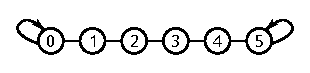
\includegraphics[scale=1.5]{gambler_line}
\end{center}
\[
T = \bordermatrix{~ & 1   & 2   & 3   & 4 \cr
                  1 & 0   & 0.5 & 0   & 0 \cr
                  2 & 0.5 & 0   & 0.5 & 0 \cr
                  3 & 0   & 0.5 & 0   & 0.5 \cr
                  4 & 0   & 0   & 0.5 & 0 \cr}
~E = \begin{pmatrix}
1.6 & 1.2 & 0.8 & 0.4 \\
1.2 & 2.4 & 1.6 & 0.8 \\
0.8 & 1.6 & 2.4 & 1.2 \\
0.4 & 0.8 & 1.2 & 1.6
\end{pmatrix}
\]
\[
F = \begin{pmatrix}
0.375 & 0.5 & 1/3 & 0.25 \\
0.75 & 1.75/3 & 1.9/3 & 0.5 \\
0.5 & 1.9/3 & 1.75/3 & 0.75 \\
0.25 & 1/3 & 0.5 & 0.375
\end{pmatrix}
\]
\end{frame}

\begin{frame}{Branching process}
In the beginning, there're $X(0)$ life forms, 
each life form has probability $p_i$ of becoming $i$ life forms in the next step.
\begin{itemize}
\item state 0 is recurrent (absorbing).
\item if $p_0 > 0$, all other states ($1,2,\ldots$) are transient since\\
	$P(X(t+1)=0|X(t)=i) = {p_0}^i > 0$
\end{itemize}
We'll show that
\[
E[X(n)] = \mu^n \cdot X(0)
\]
where
\[
\mu = \sum_{j \geq 1} j \cdot p_j = E[Z_k]
\]
and $Z_k$ is the number of offspring of the $k$-th life form, all $Z_k$ are i.i.d.
\end{frame}

\begin{frame}{Proof}
\begin{align*}
E[X(n)] & = E[E[X(n)|X(n-1)]] \\
& = E\left[E\left[\sum_{k=1}^{X(n-1)} Z_k | X(n-1)\right]\right] \\
& = E[X(n-1) \cdot \mu] \\
& = \mu \cdot E[X(n-1)] \\
& = \mu^n \cdot X(0)
\end{align*}
\end{frame}

\begin{frame}{Probability of extinction}
\begin{definition}
$e_i$ is the probability of extinction when $X(0) = i$.
\end{definition}
\textbf{Case 1:} $\mu < 1$
\begin{align*}
1 - e_i & = \lim_{n\to\infty} P(X(n) \geq 1 | X(0) = i) \\
& = \lim_{n\to\infty} \sum_{j \geq 1} P(X(n) = j|X(0) = i) \\
& \leq \lim_{n\to\infty} \sum_{j \geq 1} j \cdot P(X(n) = j|X(0) = i) \\
& = \lim_{n\to\infty} E[X(n)|X(0)=i] \\
& = \lim_{n\to\infty} \mu^n \cdot i = 0
\end{align*}
\end{frame}

\begin{frame}{Probability of extinction (cont.)}
\textbf{Case 2:} $\mu \geq 1$ 
\[
e_2 = {e_1}^2,\quad  e_3 = e_2 \cdot e_1,\quad\ldots
\]
\begin{align*}
e_1 & = P(\text{extinct}|X(0) = 1) \\
& = \sum_{j \geq 0} P(\text{extinct}|X(1) = j) \cdot P_{1j} \\
& = \sum_{j \geq 0} e_j \cdot p_j \\
& = \sum_{j \geq 0} {e_1}^j \cdot p_j
\end{align*}
We then solve the above equation to get $e_1$.
\end{frame}

\begin{frame}{Example}
\begin{align*}
& p_0 = p_1 = 0.25,\quad p_2 = 0.5 \\
\implies & \mu = 1 \cdot 0.25 + 2 \cdot 0.5 > 1 \\
\implies & e_1 = {e_1}^0 \cdot 0.25 + {e_1}^1 \cdot 0.25 + {e_1}^2 \cdot 0.5 \\
\implies & e_1 = \{1/2,~1\}
\end{align*}
Since $\mu > 1$, we know $\lim_{n\to\infty} E[X(n)] = \infty$.\\
But if $e_1 = 1$, we have $\lim_{n\to\infty} P(X(n) = 0) = 1$, which would not make $\lim_{n\to\infty} E[X(n)] = \infty$, hence $e_1 \neq 1$.
\end{frame}

\begin{frame}{Reversed Markov chain}
\begin{definition}
Let $\mathbb{X}$ (resp. $\mathbb{Y}$) be a Markov chain with matrix $P$ (resp. $Q$).\\
We say that $\mathbb{Y}$ is the \textit{reversed chain} of $\mathbb{X}$ if there exists a stationary distribution $\pi$ of $\mathbb{X}$ such that
\[
\pi_i \cdot Q_{ij} = \pi_j \cdot P_{ji}
\]
holds for all states $i,~ j \in S$.
\end{definition}
\end{frame}

\begin{frame}{Observation 1}
\begin{obs}
The reversed sequence $\mathbb{Y}$ of $\mathbb{X}$ is a Markov chain.
\end{obs}
\end{frame}

\begin{frame}{Proof}
\begin{align*}
& P(Y(n) = i_0 | Y(n-1) = i_1, Y(n-2) = i_2, \ldots , Y(n-k) = i_k) \\
= & P(X(n) = i_0 | X(n+1) = i_1, X(n+2) = i_2, \ldots , X(n+k) = i_k) \\
= & \frac{P(X(n) = i_0, X(n+1) = i_1, \ldots , X(n+k) = i_k)}{P(X(n+1) = i_1, \ldots , X(n+k) = i_k)} \\
= & \frac{P(X(n)=i_0)\cdot P(X(n+1)=i_1|X(n)=i_0)\cdot P_{i_1 i_2}\cdots P_{i_{k-1}i_k}}{P(X(n+1)=i_1)\cdot P_{i_1 i_2}\cdots P_{i_{k-1}i_k}} \\
= & \frac{P(X(n)=i_0, X(n+1)=i_1)}{P(X(n+1)=i_1)} \\
= & P(X(n)=i_0|X(n+1)=i_1) \\
= & P(Y(n)=i_0|Y(n-1)=i_1)
\end{align*}
\end{frame}

\begin{frame}{Observation 2}
\begin{obs}
If $\mathbb{Y}$ is the reversed sequence of Markov chain $\mathbb{X}$ and $\pi$ is a stationary distribution of $\mathbb{X}$, then
\[
\pi_i \cdot Q_{ij} = \pi_j \cdot P_{ji}
\]
holds for all $i,j \in S$, where $Q$ is the transition matrix of $\mathbb{Y}$.
\end{obs}
\end{frame}

\begin{frame}{Proof}
Let $\mathbb{X}$ and $\mathbb{Y}$ have distribution $\pi$
\begin{align*}
\pi_i \cdot Q_{ij} & = P(Y(n-1)=i)\cdot P(Y(n)=j|Y(n-1)=i) \\
& = P(Y(n-1)=i, Y(n)=j) \\
& = P(Y(n-1)=i|Y(n)=j)\cdot P(Y(n)=j) \\
& = P(X(n+1)=i|X(n)=j)\cdot P(X(n)=j) = \pi_j \cdot P_{ji}
\end{align*}
\end{frame}

\begin{frame}{Observation 3}\label{obs3}
\begin{obs}
Let $P$ (resp. $Q$) be the transition matrix of $\mathbb{X}$ (resp. $\mathbb{Y}$),
if vector $\pi$ satisfy the following
\begin{itemize}
\item $\sum_{i\in S} \pi_i = 1$
\item $\pi_i \geq 0 \quad\forall i \in S$
\item $\pi_i \cdot Q_{ij} = \pi_j \cdot P_{ji} \quad\forall i,j \in S$
\end{itemize}
then $\mathbb{Y}$ is the reversed sequence of $\mathbb{X}$.
\end{obs}
\begin{itemize}
\item The long-run proportion of $i\to j$ in the sequence of $\mathbb{Y}$ is equal to the long-run proportion of $j\to i$ in the sequence of $\mathbb{X}$.
\item Reversed Markov chain is the reversed sequence.
\end{itemize}
\end{frame}

\begin{frame}{Proof}
From the third property, we have
\[
\sum_{j\in S} \pi_i \cdot Q_{ij} = \pi_i = \sum_{j\in S} \pi_j \cdot P_{ji} \quad\forall i \in S
\]
From the 2nd equation, we know that $\pi \times P = \pi$, hence $\pi$ is a stationary distribution of $\mathbb{X}$.

Then by observation 2, we know that for any $\pi$, there's a reversed sequence $\mathbb{Y}'$, whose transition matrix $Q'$ satisfy
\[
\pi_i \cdot Q_{ij}' = \pi_j \cdot P_{ji} \quad\forall i,j \in S
\]
hence $\mathbb{Y} = \mathbb{Y}'$, which is a reversed sequence of $\mathbb{X}$.
\end{frame}

\begin{frame}{Example: Bulb's life}
\begin{center}

\includegraphics[scale=0.1]{light_bulb_1.png}
\end{center}
There's a room which need to be lighted by one bulb, when the bulb in use fails, it will be replaced by a new one on next day.
\begin{itemize}
\item $X(n) = i$ if the bulb in use on day $n$ is in its $i$th day of use.
\item $L$ is a random variable representing the lifetime of a bulb.
\end{itemize}
We want to know the stationary probability $\pi_i$ of state $i$.
\end{frame}

\begin{frame}{Example: Bulb's life (cont.)}
$\mathbb{X}$ is a irreducible, positive recurrent, aperiodic Markov chain which has the sequence like this:
\[
1,2,3,1,2,3,4,5,1,1,2,1,2,3,4,\ldots
\]
We know that
\[
P_{i1} = P(\text{buld, on its $i$th day of use, fails}) = \frac{P(L=i)}{P(L\geq i)} = 1 - P_{i(i+1)}
\]
And the expected return time of state $1$ is $E[L]$, which means that the long-run proportion of state $1$ is $1/E[L]$ by page \pageref{pro_value}.
\end{frame}

\begin{frame}{Example: Bulb's life (cont.)}
Take $\mathbb{Y}$ (with matrix $Q$) as the reversed chain of $\mathbb{X}$, we know that for all $i\in S$,
\begin{itemize}
\item $Q_{(i+1)i} = 1$
\item $Q_{1i} = P(L = i)$
\item $\pi_1\cdot Q_{1i} = \pi_i\cdot P_{i1}$
\end{itemize}
Hence,
\[
\pi_i = \frac{\pi_1\cdot Q_{1i}}{P_{i1}} = 
\frac{P(L=i)\cdot P(L\geq i)}{E[L]\cdot P(L=i)} = \frac{P(L\geq i)}{E[L]}
\]
\end{frame}

\begin{frame}{Time-reversible}
\begin{definition}
$\mathbb{X}$ is \textit{time-reversible} if $\mathbb{X}$ is the reversed chain of $\mathbb{X}$.
\end{definition}
\end{frame}

\begin{frame}{Example: Reversed drunken man}
\begin{center}
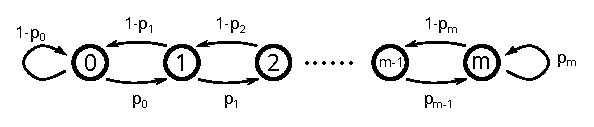
\includegraphics[scale=1.0]{drunken_man}
\end{center}
\begin{itemize}
\item $0 < p_0\leq 1$
\item $0\leq p_m < 1$
\item $0 < p_i < 1 \quad\forall i = 1,\ldots,m-1$
\end{itemize}
The long-run proportion of transition $i\to i+1$ and $i+1\to i$ are the same, since one must go back to $i$ from $i+1$ in order to go to $i+1$ from $i$.\\
Hence the drunken man problem is time-reversible.
\end{frame}

\begin{frame}{Example: Reversed drunken man (cont.)}
\begin{align*}
\pi_0\cdot p_0 &= \pi_1\cdot (1-p_1)\\
\pi_1\cdot p_1 &= \pi_2\cdot (1-p_2)\\
&\vdots \\
\pi_{m-1}\cdot p_{m-1} &= \pi_m\cdot (1-p_m)
\end{align*}
Thus,
\begin{align*}
\pi_1 & = \pi_0\cdot p_0/(1-p_1) \\
\pi_2 & = \pi_1\cdot p_1/(1-p_2) \\
& \vdots \\
\pi_m & = \pi_{m-1}\cdot p_{m-1}/(1-p_m)
\end{align*}
\end{frame}

\begin{frame}{Example: Reversed drunken man (cont.)}
\begin{align*}
& \pi_i = \underbrace{\frac{\prod_{j=0}^{i-1}p_j}{\prod_{j=1}^{i}(1-p_j)}}_{q_i}\cdot \pi_0 
	\quad\forall i=1,\ldots m \\
\implies & \pi_0 + \sum_{i=1}^m \pi_i = 1 = \pi_0 + \sum_{i=1}^m q_i\cdot \pi_0 \\
\implies & \pi_0 = \frac{1}{1 + \sum_{i=1}^m q_i} \\
\implies & \pi_k = \frac{q_k}{1 + \sum_{i=1}^m q_i} \quad\forall k=0,1,\ldots m
\end{align*}
\end{frame}

\begin{frame}{Example: Two bukkits of balls}
There're two bukkits contain total $m$ balls.\\
In each step, we randomly choose one ball and put it in another bukkit.\\
Let $X(n)$ represent the number of balls in the first bukkit, it's the Markov chain of previous example with
\[
p_0 = 1,~p_m = 0,~p_i = \frac{m-i}{m} \quad\forall i=1,\ldots,m-1
\]
We can get that
\[
q_i = \frac{\prod_{j=0}^{i-1}\frac{m-j}{m}}{\prod_{j=1}^{i}\frac{j}{m}} = 
\frac{\prod_{j=0}^{i-1}m-j}{\prod_{j=1}^{i}j} = \binom{m}{i} \quad\forall i=1,\ldots m
\]
\[
\implies \pi_0 = \frac{1}{1 + \sum_{i=1}^m \binom{m}{i}} = 
\frac{1}{2^m} \implies \pi_k = \frac{\binom{m}{k}}{2^m} \quad\forall k=0,1,\ldots m
\]
\end{frame}

\begin{frame}{Example: A random walk}
\begin{columns}
\begin{column}{0.4\textwidth}
\begin{center}
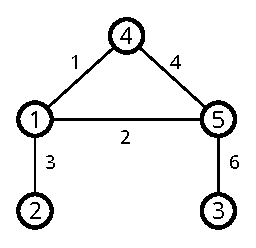
\includegraphics[scale=1.0]{random_walk}
\end{center}
\end{column}
\begin{column}{0.6\textwidth}
\[
P_{ij} = \frac{w(i,j)}{\sum_k w(i,k)}
\]
where $w(a,b)$ is the weight of edge $(a,b)$.\\
To make it as a time-reversible chain, we let
\[
\pi_i = \frac{\sum_k w(i,k)}{\sum_\ell \sum_k w(\ell,k)} \quad\forall i
\]
We can see that
\[
\pi_i\cdot P_{ij} = \pi_j\cdot P_{ji} \quad\forall i,j
\]
\end{column}
\end{columns}
\end{frame}

\begin{frame}{Hastings-Metropolis sampling algorithm}
Design an irreducible Markov chain $\mathbb{X}$ such that the unique stationary distribution of $\mathbb{X}$ is the distribution of random variable $Y$.\\
Since the long-run proportion of state $i$ is $P(Y=i)$,
\[
\lim_{n\to\infty} \frac{X(1)+X(2)+\ldots+X(n)}{n} = \sum_{i\in S} i\cdot P(Y=i) = E[Y] = \mu
\]

While computing $\mu$ by the law of large number is difficult (hard to sample on $Y$), we use this alternative method to compute $\mu$ by generating a sequence of $\mathbb{X}$, which is sometime easier.
\end{frame}

\begin{frame}{Hastings-Metropolis sampling algorithm (cont.)}\label{possible_Y}
There's a random variable $Y$ such that
\[
P(Y=i) = \frac{b_i}{C}
\]
for some unknown (or intractable) $C = \sum_{i\in S}b_i$.\\
We then design a Markov chain $\mathbb{X}$ that
\begin{itemize}
\item $P_{ii} = Q_{ii} + \sum_{k\in S, k\neq i} Q_{ik}\cdot (1-q_{ik})$
\item $P_{ij} = Q_{ij}\cdot q_{ij} \quad\forall j\neq i$
\end{itemize}
where
\begin{itemize}
\item $Q$ is the transition matrix of an arbitrary irreducible Markov chain $\mathbb{X}$ which has the same state space as $Y$.
\item $q$ is a matrix to be determined later.
\end{itemize}
\end{frame}

\begin{frame}{Hastings-Metropolis sampling algorithm (cont.)}
For $n = 0,1,\ldots$,
\begin{enumerate}
\item If $X(n)=i$, set $Z$ such that $P(Z = j) = Q_{ij} \quad\forall j\in S$.
\item If $Z = j$, set $X(n+1)$ such that
	\begin{itemize}
	\item $P(X(n+1)=j) = q_{ij}$
	\item $P(X(n+1)=i) = 1 - q_{ij}$
	\end{itemize}
\end{enumerate}
One can see that this satisfies the requirement on previous page.
\end{frame}

\begin{frame}{Hastings-Metropolis sampling algorithm (cont.)}
Then, we let
\begin{align*}
& q_{ij} = \min\left( \frac{b_j\cdot Q_{ji}}{b_i\cdot Q_{ij}}, 1 \right) \\
\implies & b_i\cdot Q_{ij}\cdot q_{ij} = b_j\cdot Q_{ji}\cdot q_{ji} \\
\implies & \frac{b_i}{C}\cdot P_{ij} = \frac{b_j}{C}\cdot P_{ji}
\end{align*}
By observation 3 on page \pageref{obs3}, we know that $(b_1/C, b_2/C,\ldots)$ is the stationary distribution of $\mathbb{X}$.
\end{frame}

\begin{frame}{Example: Space of permutations}
\begin{example}
Let $S$ consist of all the permutations $(x_1, x_2, \ldots, x_n)$ of $\{1,2,\ldots,n\}$ that
\[
\sum_{k=1}^n k\cdot x_k \geq \frac{n^3}{4}
\]
\end{example}
\begin{itemize}
\item This is same as $Y$ in page \pageref{possible_Y} with $C=|S|$ and $b_i = 1 ~\forall i$.
\item $S$ is hard to compute.
\item We need to design a matrix $Q$ such that when given a permutation $x$, it's efficient to compute the value of $Q_{xy} ~\forall y\in S$.
\end{itemize}
\end{frame}

\begin{frame}{Example: Space of permutations (cont.)}
We let
\[
Q_{xy} = \frac{1}{N(x)} \quad,\text{if $y$ can be obtained from $x$ by one swap}
\]
where $N(x)$ is the number of permutations that can be obtained from $x$ by one swap.
For example:
\[
\underbrace{(1,2,3,4,5)}_y \leftrightarrow 
\underbrace{(1,3,2,4,5)}_x \leftrightarrow 
\underbrace{(1,3,4,2,5)}_y
\]
This chain is irreducible since each $x\in S$ can go to $(x_1,x_2,\ldots,x_n)$, where $x_1 \leq x_2 \leq \ldots \leq x_n$, by several swaps.\\
Also, given a $x$, finding all the obtainable $y$ can be done efficiently.
\end{frame}

\end{document}

